\documentclass[twocolumn]{article}

% Language and font encodings
\usepackage[english]{babel}
\usepackage[utf8x]{inputenc}
\usepackage[T1]{fontenc}
\usepackage{enumitem}
\usepackage{amsthm}
\usepackage[twocolumn, top=3cm, bottom=2cm, left=2cm, right = 2cm, marginparwidth=1.75cm]{geometry}

\newtheorem*{sos*}{Solution Space}
\newtheorem*{op*}{Optimization}
\newtheorem*{ml*}{Machine Learning}
\newtheorem*{he*}{Heuristic}
\newtheorem*{me*}{Meta-Heuristic}
\newtheorem*{ga*}{Genetic Algorithm (GA)}
\newtheorem*{pso*}{Particle Swarm Optimization (PSO)}



%useful packages
\usepackage{amsmath}
\usepackage{graphicx}
\usepackage[colorinlistoftodos]{todonotes}
\usepackage[colorlinks=true, allcolors = blue]{hyperref}
\title{Genetic Algorithm Particle Swarm Optimization Hybridization}
\author{Daniel Khalil
\\\texttt{Computer Science}
\\\texttt{Daytona Beach, Florida}
\\\texttt{600 South Clyde Morris Blvd.} \and
Luke Crump
\\\texttt{Computer Science}
\\\texttt{Daytona Beach, Florida}
\\\texttt{600 South Clyde Morris Blvd.} \and
Keith Garfield
\\\texttt{Computer Science}
\\\texttt{Daytona Beach, Florida}
\\\texttt{600 South Clyde Morris Blvd.}
}

\begin{document}
\maketitle
\begin{abstract}
This research explored hybridizing Particle Swarm Optimization (PSO) and Genetic Algorithms (GA). Computational efficiency and quality of solution were measured for multiple hybrid variations. It was found that the the hybrid algorithm performed slightly better than PSO and GA in x/x tests when executed on solution spaces with many local minimums.
\end{abstract}
\section{Introduction}
Heuristic optimization techniques have become a widespread technique within the field of machine learning [1]. Applications extend to training Neural Networks, approximating solutions to NP-Complete problems, pattern recognition, and Heuristic evolutionary optimization algorithms such as Genetic Algorithms (GA) and Particle Swarm Optimization (PSO). The concept of meta-heuristics proposes that "it is often sufficient to find an approximate or partial solution"[1]. By sacrificing accuracy, these algorithms gain efficiency. Although defining the scope of all possible solutions determines the accuracy of heuristic algorithms. If the solution space becomes larger or deceptively holds multiple viable solutions, the disadvantage of using meta-heuristics becomes the increasing loss of accuracy.

Population-based Meta-Heuristic algorithms have tools such as GA's mutation rate and PSO's cognitive and social components that allow exploration of a given solution space. These tools allow for convergence on optimal solutions even within solution spaces with multiple local minimums or maximums. The hybrid algorithm proposed includes both the exploration and convergence components of GA and PSO together. This research tests whether this combination will enact a positive effect on the efficiency and quality of the result. There have been various implementations of hybridization between meta-heuristic algorithms [2][3][7] This research explores yet another implementation and/or perspective into the hybridization of two meta-heuristic algorithms.

\subsection{Definitions}


\begin{sos*}
The set of all possible solutions to a specific problem. (right or wrong)
\end{sos*}

\begin{op*}
The process of finding the best solution or solutions out of a range of possible solutions.
\end{op*}

\begin{ml*}
a subset of Artificial Intelligence that is intended to allow an algorithm to learn and improve performance from experiences in an environment. 
\end{ml*}

\begin{he*}
A problem dependent algorithm that is faster and more efficient than traditional methods by sacrificing accuracy, or completeness.
\end{he*}

\begin{me*}
A high-level problem independent algorithm that uses heuristic methods to allow application to a broad variety of problems.
\end{me*}

\begin{ga*}
a metaheuristic technique that utilizes evolution of solutions based off of survival of the fittest.
\end{ga*}

\begin{pso*}
A metaheuristic technique that utilizes the movement of solutions based off of communication of other solutions within a solution space.
\end{pso*}

\section{Genetic Algorithm}
Genetic Algorithm (GA) are an evolutionary metaheuristic optimization algorithm based on Darwin's theory of evolution. The algorithm initially constructs a population p containing $p_i$ which is a vector containing random solutions between the solution space's minimum boundary and maximimum boundary then follows steps 1-4 for each $p_i \epsilon p$
\begin{enumerate}



    \item \textbf{Evaluation}
Evaluation includes for each $p_i \epsilon p$ assign a fitness value based on the location of $p_i$ in the solution space. in the case of this research $eval(p_i) = f(p_i)$ \\f(x) = a given benchmark function.

    \item \textbf{Selection}
Selection includes a picking favorable $p_i \epsilon p$ to breed new solutions based off of a $p_i$'s evaluation or fitness. In this research the Tournament selection method was used:
		\begin{enumerate} [label=(\alph*)]
        \item pick two solutions randomly from p ($p_i$, $p_j$)
        \item if eval($p_i$) > eval($p_j$): then: return $p_i$
else: return $p_j$
\end{enumerate}

\begin{figure}[!h]
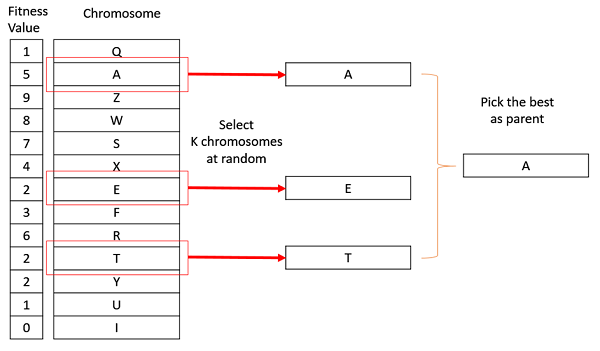
\includegraphics[scale=0.5]{Images/tournament.png}
\caption{Tournament Selection}
\end{figure}


Selection is run twice to return two viable parents for crossover. 

\item \textbf{Crossover}
Crossover includes breeding two parent solutions together to create a child of those two solutions. The purpose of crossover or blending solutions together, is to allow convergence to a point within a solution space. In this research a real number variation of the crossover algorithm was chosen to be BLX (blended crossover).\\

BLX is a method of crossover that blends real number solutions[10]. with parents $x_i$ and $y_i$ for each offspring generated $d_i = $ | $x_i - y_i $ |\\

generate $u$, a random number within the range: \\
$$ [ min (x_i, y_i) - a * d_i, max(x_i, y_i) + a * d_i ] $$
$x_i' = u$ is the newly generated individual of the next population.

$$ x_i \in P_{generation1} , y_i \in P_{generation1} $$
$$ \exists x_i' \in P_{generation2} , x_i' = u $$ 

$a$ is a parameter to the blx algorithm that was chosen as $0.1$.

\begin{figure}[h!]
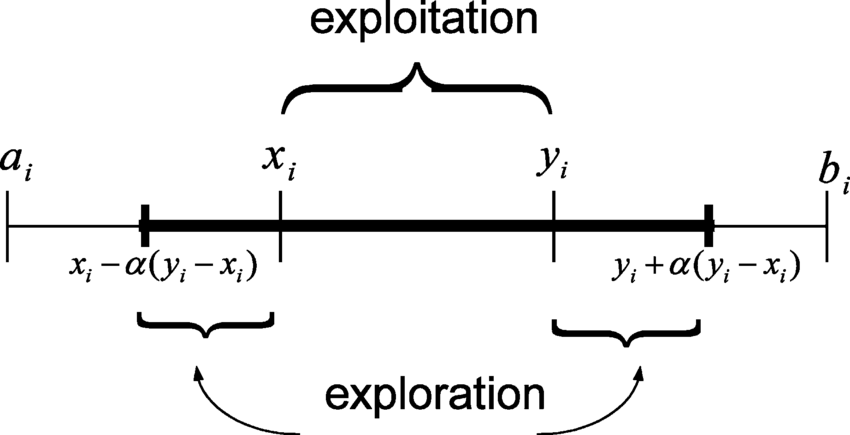
\includegraphics[scale=0.26]{Images/blx.png} 
\caption{BLX Visual}
\end{figure}


\item \textbf{Mutation}
Mutation provides diversity to each new generation, so it doesn't get trapped in deceptive cases. In this research pi has a chance to be multiplied by a floating-point value that is between zero and two.

Repeating these steps until an optimal solution has been found, Genetic Algorithms eventually converges the entire population to a solution inside the solution space.

The critical aspects of how GAs find a solution is in how they explore and converge. Exploration is affected by the selection and mutation methods of GA and is essential to help the population not get trapped in a local minimum or maximum. Convergence is affected by the selection and crossover methods of GA and is essential to moving the entire population towards a specific solution.
\end{enumerate}

\section{Particle Swarm Optimization}

Particle Swarm Optimization (PSO) is a metaheuristic optimization algorithm based off the social behavior of birds[3]. PSO uses a vector equation that uses the position of the specific particle, the position of the best particle, and randomness to explore and converge on a solution. through iterations called epochs.


The algorithm initially constructs a population of particles that contain a random solution between the upper and lower bounds of the solution space, assigns each particle a random velocity vector vi within the bounds of the solution space.\\


\textbf{$gBest$} - the swarm’s global best position within the solution space\\

\textbf{$pBest$} - a particle’s personal best position within the solution space \\

\textbf{$\omega$} - inertia parameter (normally between 0.6-0.9)\\

\textbf{$\varphi _p$} - social component parameter (normally 2)\\

\textbf{$\varphi _g$} - cognitive component parameter \\(normally = $\varphi _p$ = 2)\\

r - random number between 0-1\\

\begin{enumerate}


    \item \textbf{Evaluation}
Evaluates the particle’s solution: xi

    \item \textbf{Update-pBest}
If the particle’s solution is better, then it’s personal best it updates that particles personal best: $p_i$

    \item\textbf{ Update-Swarm’s-gBest}
If the particle’s solution is the best solution out of the entire swarm then the global best solution is updated $g_d$

    \item \textbf{Update each particles velocity}
$$v_i,d ← \omega v_i,d + \varphi _p r_p (p_i,d-x_i,d) + \varphi_ g r_g (g_d-x_i,d)$$


\begin{figure}[h!]
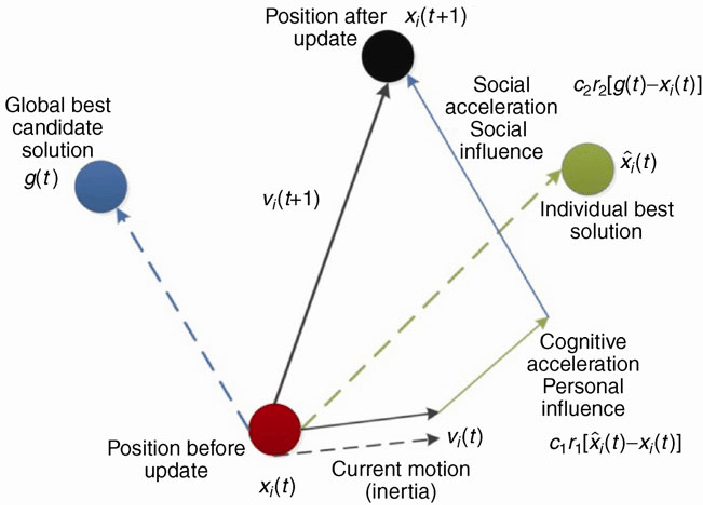
\includegraphics[scale=0.3]{Images/PSO.png} 
\caption{Particle Swarm Vector Calculation}
\end{figure}


    \item \textbf{Updates particle’s position}
 	$$p_i ← p_i + v_i,d$$
\end{enumerate}

These steps repeat for each particle for each epoch. To promote convergence the velocity vector equation uses the social component to move each of the particles towards the global best solution, to promote exploration of the solution space the random parameter r is multiplied to each component of the equation, as well as the inertia parameter $\omega$.

\section{Hybrid Algorithm}

To test the affects of hybridization of PSO and GA. GA, and PSO will be tested against 2 different hybrid algorithms. If these algorithms are awarded a higher fitness, in a shorter amount of iterations it will be accepted that these algorithms perform better than the nonhybrid versions of GA or PSO.

The proposed hybridization will combine both the exploration techniques of PSO and GA together by utilizing the particles of PSO and the individuals of GA all within the same population. Although they will not run seperately, the exploration techniques of both algorithms will be pulling information such as parents, and global best's from the entire population containing both particles and chromosomes.\\

\begin{enumerate}


    \item \textbf{Instantiate}:
    
construct a population P of random solutions vectors $p_i$ within the bounds of a solution space.

    \item \textbf{ Encapsulate a percentage of Particles}
    
encapsulate a percentage $\mu$ [0,1] of $p_i \epsilon P$ within a set of particles $V$ that contains a personal best and global best as well as a velocity vector. \\
$P = $ set of all particles
$$P_{particles} \subseteq P , P_{genome} \subseteq P $$
$$P_{particles} \cup P_{genome} = P$$
$$ \dfrac{|P_{particles}|}{|P|} = \mu$$


\end {enumerate}

For each Generation:

\begin{enumerate}[label=\alph*]


    \item  \textbf{Update pBest}
    
for each of the Particles contained in the population, update the attribute pBest. if the position is evaluated to be less than the current pBest.\\
$\forall p \in P_{particles}$ | $(eval(p_{location}) < eval(p_{pBest})) \Rightarrow$

$p_{pBest} = p_{location}$ 

    \item \textbf{Update gBest (from entire population)}
    
Global best updates to the position of an individual if and only if an individual's location pulled from the entire population is less than the current gBest

$\exists p \in P $ | $g = p_{location}$ | $eval(g) < eval(gBest) \Rightarrow$
$gBest = p_{location}$
    \item  \textbf{Update Allocated Particle Velocities}
    
for each of the particles in the particle population set the particles velocity equal to the equation from particle swarm.
$$\forall p \in P_{particles}$$
$$p_{v},d ← \omega v_i,d + \varphi _p r_p (p_i,d-x_i,d) + \varphi_ g r_g (g_d-x_i,d)$$
    \item \textbf{Update Allocated Particle Positions}
    
for each of the particles in the particle population set the particles position equal to the equation from particle swarm\\
$\forall p \in P_{particles} $ | $p ← p + p_v,d$
\item \textbf{Select Parents (from entire population)}
    
For each individual in the $P_{genome}$ select 2 parents from P via tournament method.

\item \textbf{Crossover}
    
For each individual in $P_{genome}$ crossover using the parents from selection via BLX to produce children in $P_{genome}$

\item \textbf{Mutation}

For each individual in $P_{genome}$ mutate based off of a fixed mutation rate.

\end{enumerate}

These steps will repeat to converge to a solution.\\
\begin{figure}[h!]
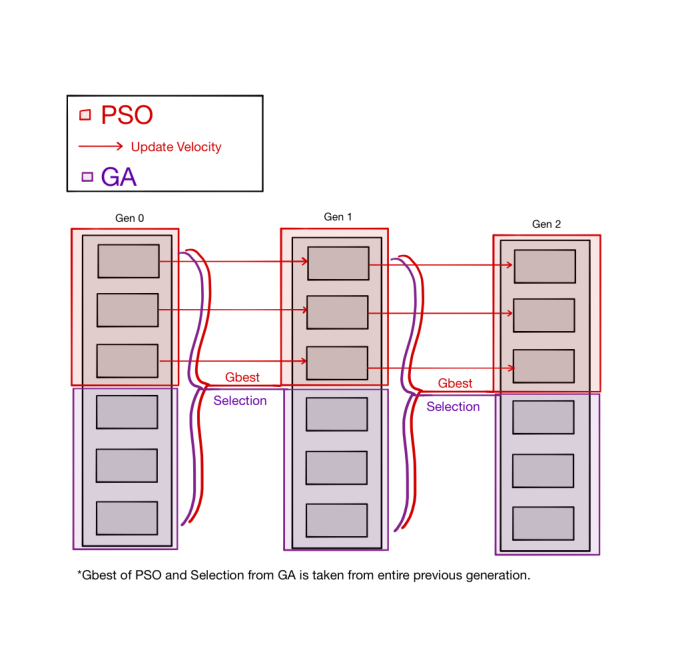
\includegraphics[scale=.35]{Images/hybridvisualization.png} 
\caption{Hybridization Visualization}
\end{figure}

%image will go here

The hybridization of PSO and GA, is to increase the exploration of the population through the solution space. As the population will utilize the exploration components of Particle Swarm Optimization (Inertia, and random aspects of the velocity calculation), as well as the exploration aspects of Genetic Algorithm, (mutation rate, and selection).

%image will go here

Adding this extra exploration aspect will hopefully allow convergence to a more optimal solution within solution spaces that contain either extra noise, or more local minimums / local maximums.

\section{Benchmark Functions}

To ensure that the algorithms were tested against a variety of situations, the benchmark functions were selected through their unique topologies. functions that were considered were ones with one or more of these features:

\begin{enumerate}

\item{multiple local minimums}

\item {multiple local maximimums}

\item {plateus}

\item {none of the above}

\end{enumerate}

\subsection{Ackleys Function}
$$f(x) = -a * exp (-b * \sqrt{\dfrac{1}{d}* \sum_{n=1}^{\infty} x_i^{2}}) - exp(\dfrac{1}{d} * \sum_{n=1}^{\infty} x_i^{2}) + a + exp(1)$$
\subsection{Eggholder Function}
$$f(x) =(x_2 + 47)sin(\sqrt{|x_2 + \dfrac{x_1}{2} + 47|})-x_1 sin ( \sqrt{|x_1-(x_2 + 47 )|})$$
\subsection{Holder Table Function}
$$f(x) = -|sin(x_1)cos(x_2)exp(|1-\dfrac{\sqrt{x_1^2 + x_2^2}}{\pi}|)|$$
\subsection{Levy Function}
$$f(x) = sin^2(\pi w_1)+ \sum_{i=1} ^{d-1}(w_i -1)^2[1+10sin^2(\pi w_i + 1)] + (w_d - 1)^2[1 + sin^2(2\pi w_d)$$

$w_i = 1 + \dfrac{x_i -1}{4},$ for all i=1, ..., $d$

\subsection{Easom Function}
$$f(x) = -cos(x_1)cos(x_2) exp(-(x_1 -\pi)^2-(x_2-\pi)^2)$$

\subsection{Rastrigin Function}
$$f(x) = 10d \sum_{i=1}^{d}[x_i^2 - 10 cos (2 \pi x_i)$$
\subsection{Sphere Function}
$$f(x) = \sum_{i=1}^{d} x_i^2$$

\section{Experimental Design}

Plotting the fitness over 20 iterations on each the 6 different optimization benchmark functions, all three algorithms are executed to understand efficiency. In this test the algorithms will be optimizing for the global minimum, so the favorable fitness of each algorithm will be the smallest value.\\

\textbf{Tests were run on benchmark functions 1-7}\\

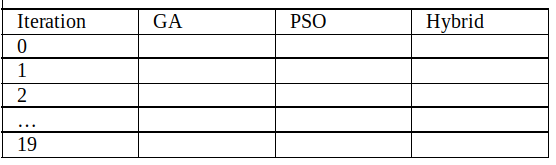
\includegraphics[scale=0.4]{Images/table.png}

(Each algorithm is executed 100 times then averaged to find the value for a specified iteration)


\begin{figure}[h!]
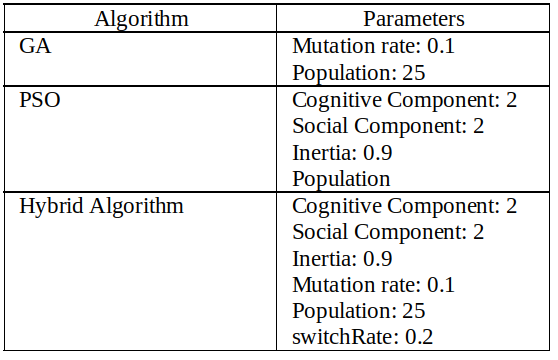
\includegraphics[scale=0.39]{Images/setvariables.png}
\caption{Chosen Variables}
\end{figure}

\section{Results}
The pattern found was that the hybrid algorithm did not outperform in benchmark functions with less prominent local minimums.

it was found that the hybrid did not outperform in benchmark functions with less prominent local minimums. For Example when compared to the other algorithms in solving Ackley's function, the hybrid algorithm recieved almost the same evaluation as PSO.
\\


%\begin{figure}[h!]
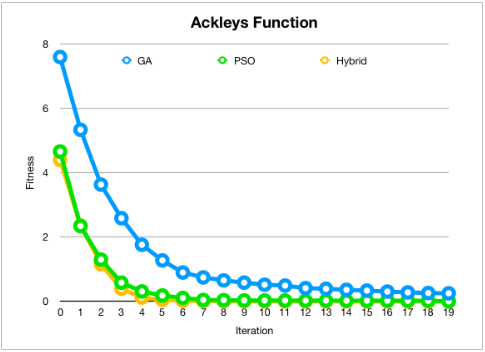
\includegraphics[scale=0.45]{Images/Ackley.png} 
%\caption{Ackley Test}
%\end{figure}

the same was found for the sphere function. The sphere function has only one global minimum and no local minimums.
\\

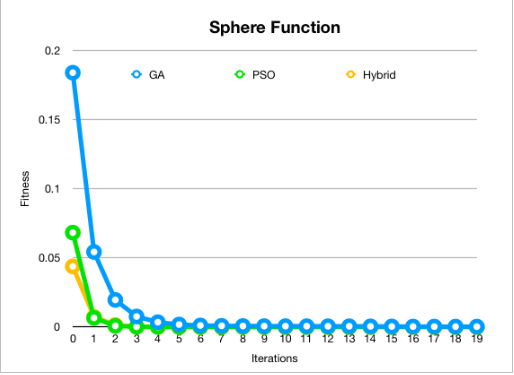
\includegraphics[scale=0.45]{Images/Sphere.png} 

Although, in functions that had many local minimums, the hybrid algorithm outperformed Genetic Algorithm and Particle Swarm Optimization. In Particular, when the Hybrid Algorithm was executed on the Rastrigin function, it converged to a solution faster then other algorithms.
\\
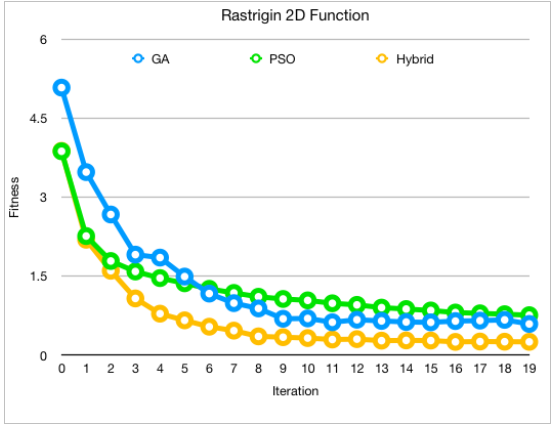
\includegraphics[scale=0.43]{Images/Rastrigin2D.png} 
\\
Increasing the dimensions of the Rastrigin function did not change this. For example for the 6 Dimensional Rastrigin function they hybrid was still outperforming the other algorithms.
\\
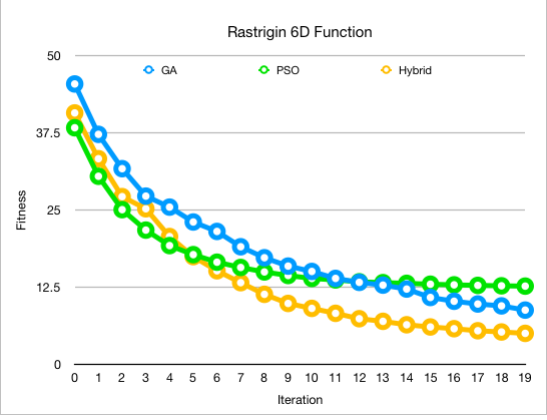
\includegraphics[scale=0.43]{Images/Rastrigin.png} 
\\
To check how the hybrid algorithm would perform on solution spaces that contained plateaus; the GA, PSO and the hybrid algorithm were executed using the Easom function which has a large area containing a plateau.
\\
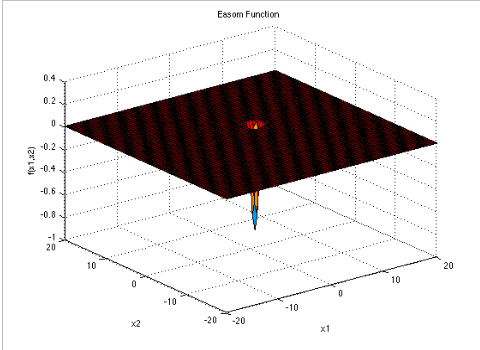
\includegraphics[scale=0.43]{Images/Easomview.png} 
\\
Easom Function visualized in 3D space
\\
The Easom function’s hybrid algorithm execution had a slightly quicker convergence speed then particle swarm optimization, although the difference was within 1-2 iterations.
\\
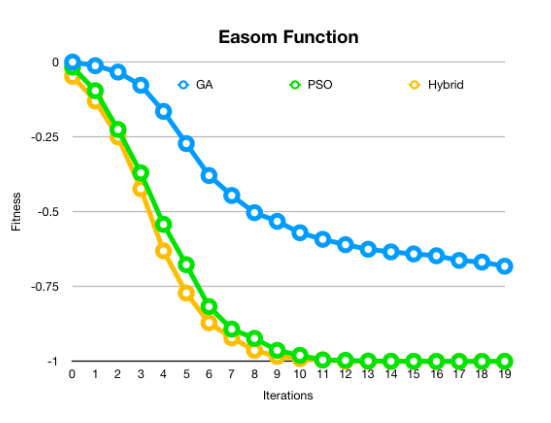
\includegraphics[scale=0.40]{Images/Easom.png} 

\section{Conclusion}

	    The proposed GAPSO hybridization outperformed GA and PSO on three different benchmark functions: the Rastrigin, Easom, and Levy function. In 4 other tests: the Egg Holder, Holder Table, Ackley, and Sphere function, the difference in convergence speed was approximately the same convergence. With the exception of the rastrigin benchmark, GAPSO did not significantly outperform GA or PSO. Although GA or PSO never significantly outperformed the hybrid, the accuracy and speed compared to the standard seemed unimpressive in all cases but Rastrigin. The hybrid optimizing the Rastrigin function was faster and more accurate in every test for every dimension.

Utilizing the given parameters for PSO and GA, 71.4\% of the tests favored PSO over GA. PSO outperformed GA in 5 out of the 7 in the given benchmark functions. The other 29.6\% favored GA over PSO on the Levy and Rastrigin function.

The intention behind the the hybrid algorithm was to blend both of the exploration features of GA and PSO into one hybrid meta-heuristic algorithm. The expectation was that combining both exploration features would expidite the convergence speed of the algorithm on more deceptive or noise filled benchmark functions. The results of testing this algorithm on a variety of benchmark functions and comparing it to GA and PSO's results. Under a specific set of functions, combining these algorithms is favorable although implementation in a broader collection of solution spaces would warrant the use of PSO.

Other research has implemented the hybridization of GA and PSO several times[2][3][4], the goal of this paper to open up another perspective on how this hybridization could be accomplished.

\section{References}

[1] Heuristic and Meta-Heuristic Algorithms and Their Relevance to the Real World: A Survey
$https://ijcert.org/ems/ijcert_papers/V2I55.pdf$


[2]PSO-GSA (Particle Swarm Optimization, Gravitational Search Algorithm Hybrid
https://ieeexplore.ieee.org/abstract/document/6141614

[3] Gene selection in cancer classification using PSO/SVM and GA/SVM hybrid algorithms
https://ieeexplore.ieee.org/abstract/document/4424483

[4]GA and a novel PSO-GA-based hybrid algorithm
https://www.sciencedirect.com/science/article/pii/S0020019004003254

[5]Variable-Length Particle Swarm Optimization for Feature Selection on High-Dimensional Classification
https://ieeexplore.ieee.org/document/8458226

[6]How efficient are genetic algorithms to solve high epistasis deceptive problems?
https://ieeexplore.ieee.org/abstract/document/4630806
    1. [7]Development and validation of different hybridization strategies between GA and PSO
https://ieeexplore.ieee.org/document/4424823

[8]Dealings with Problem Hardness in Genetic Algorithms
https://bib.irb.hr/datoteka/407953.29-202.pdf

[9]The Ant Colony Optimization Meta-Heuristic
%https://citeseerx.ist.psu.edu/viewdoc/download?doi=10.1.1.184.955&rep=rep1&type=pdf

[10]A crossover operator using independent component analysis for real-coded genetic algorithms
https://ieeexplore.ieee.org/document/934452

%\begin{table}
%\centering
%\large
%\begin{tabular}{ccc|cc}
%\hline
%No.	& Name & Function \\
%\hline
%\hline
%1 & GA & col\\
%2 & PSO & col \\
%3 & Holder Table Function & col \\

	
%\end{tabular}
%\caption{Algorithm Parameters}
%\label{tab:mylabel}
%\end{table}
	
\end{document}